%%%%%%%%%%%%%%%%%%% Figure  %%%%%%%%%%%%%%%
\begin{figure}[t]
  \begin{pspicture}(0,0)(15,17)
% Include graphs
	\rput[b](7.5,0){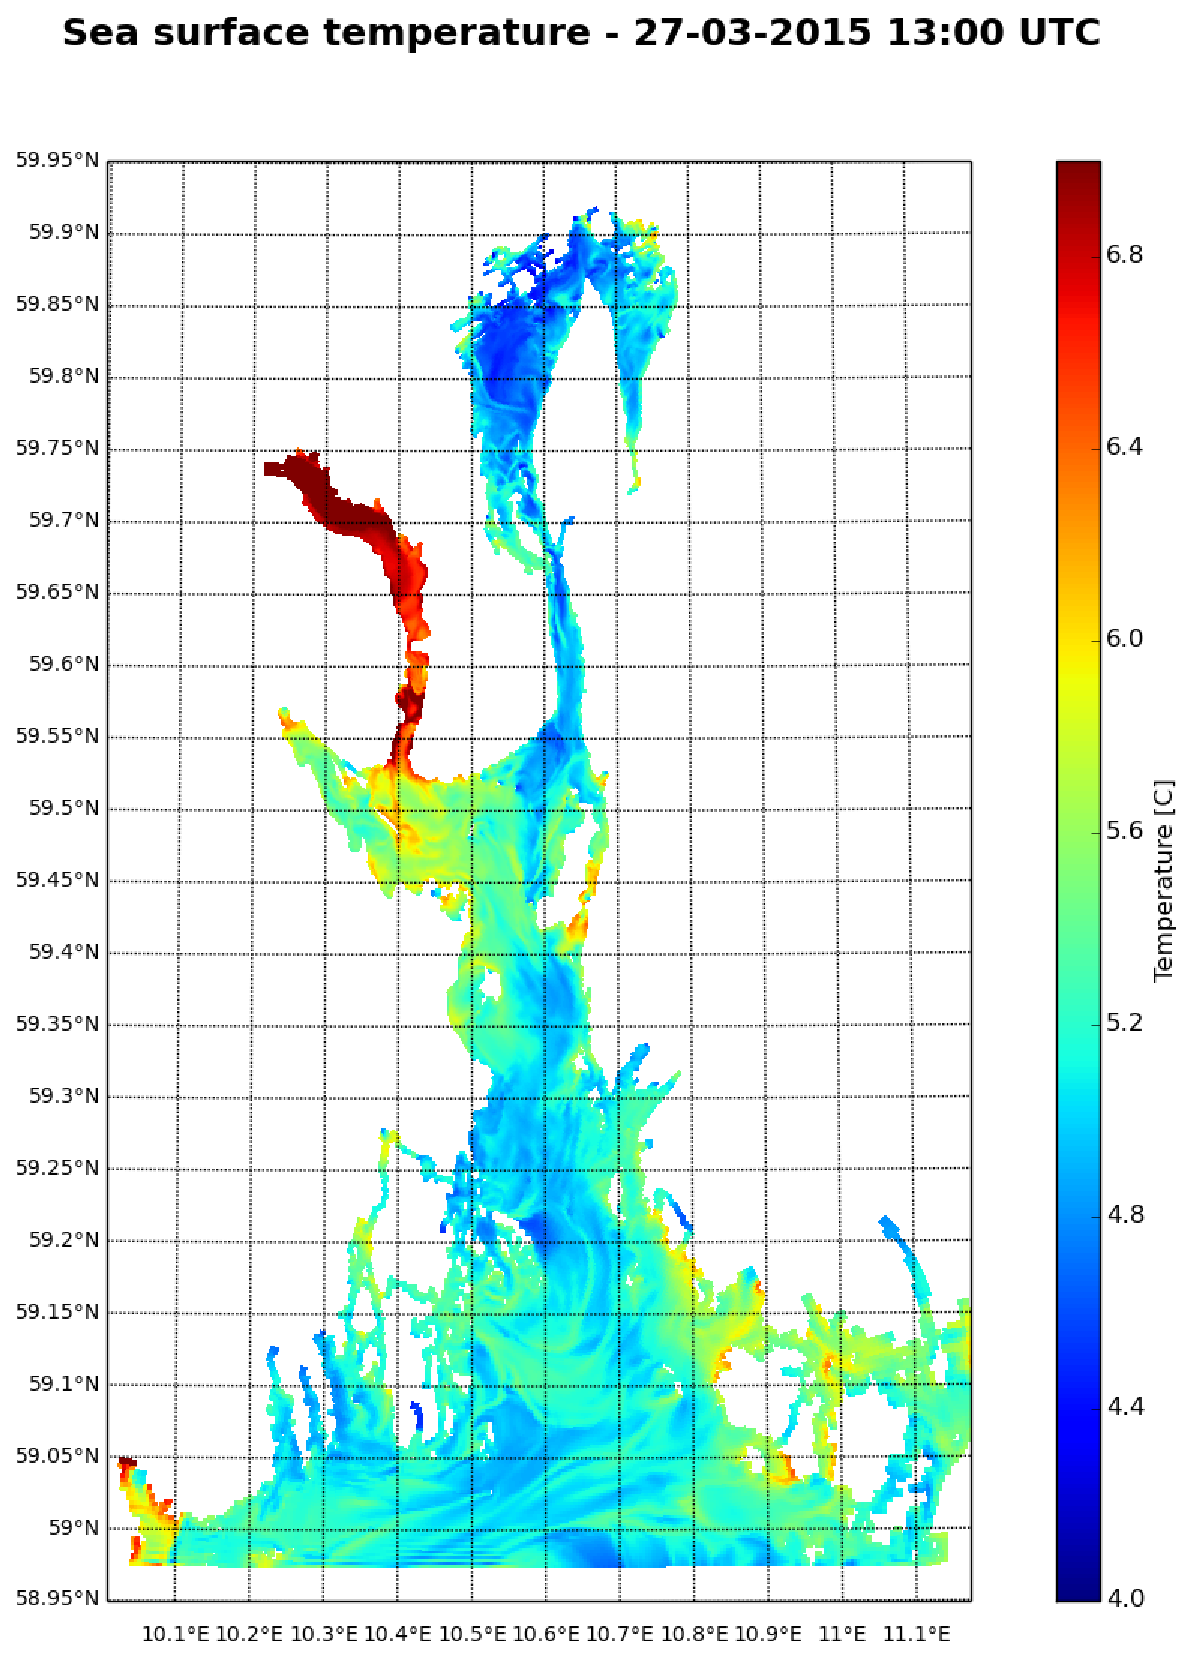
\includegraphics[height=17cm]{kap5/temp_hele_0_current_crop}}
  \end{pspicture}
  \caption{\small Sea surface temperature (SST) for the entire model domain of the FjordOs model. Note the high SST in the Drammensfjorden area. We believe this is most likely caused by the entrainment (mixing) of warmer water from below. This warm water is probably left from imperfect initial conditions. }
  \label{fig:temp_hele}
\end{figure}

